%*******************************************************
% Capitulo nueve
%*******************************************************

\chapter{Capa de Infraestructura}

\section{Infraestructura}

\marginpar{
    \begin{figure}[H]
        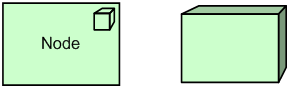
\includegraphics[scale=0.6]{Inode}
    \end{figure} 
    \footnotesize 
    \textbf{Nodo}. Un recurso computacional donde cualquier artefacto se pueden almacenar o desplegar para ejecutar.
\newline
}
\marginpar{
    \begin{figure}[H]
        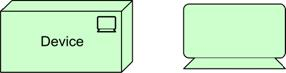
\includegraphics[scale=0.6]{Idevice}
    \end{figure} 
    \footnotesize 
    \textbf{Dispositivo}. Un recurso de hardware sobre el cual los artefactos se pueden almacenar o desplegar para su ejecución.
\newline
}

\marginpar{
    \begin{figure}[H]
        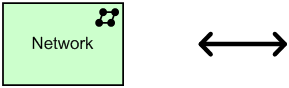
\includegraphics[scale=0.8]{Inetwork}
    \end{figure} 
    \footnotesize 
    \textbf{Red}.Un medio de comunicación entre dos o mas dispositivos.
}El punto de vista de infraestructura contiene los elementos de la infraestructura de hardware y software de apoyo a la capa de aplicación, tales como dispositivos físicos, redes o software del sistema (por ejemplo, sistemas operativos, bases de datos y middleware).

\begin{figure}[H]
\centering
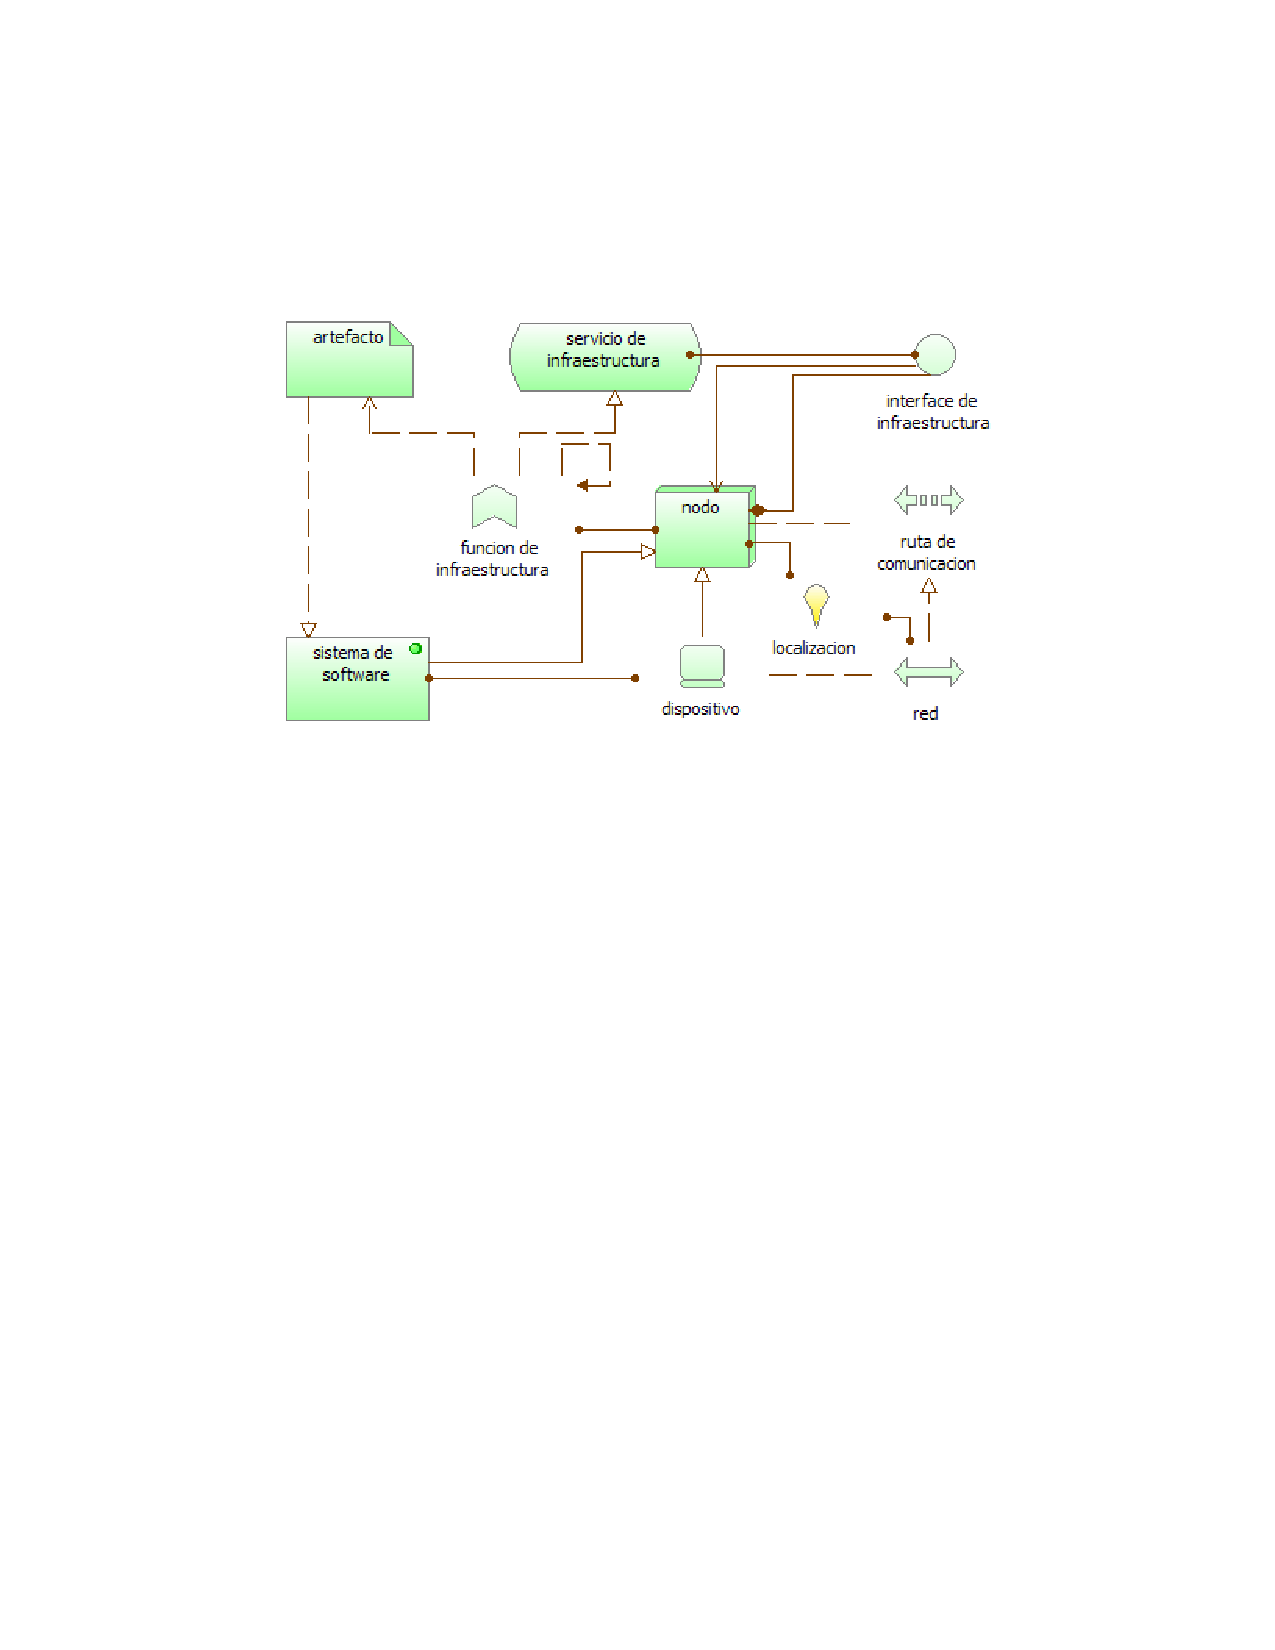
\includegraphics[scale=0.7]{infraestructura}
\caption{Metamodelo del punto de vista de infraestructura.}
\end{figure}

La propuesta actual establece un servicio escalable en cloud con un proveedor el cual esconderá los detalles del servicio. Este proceso de ocultación incluye el ámbito completo de servicio conectividad, desempeño, y todos los aspectos de operación de la infraestructura.

Se propone entonces un uso de infraestructura sin detalle pero orientado a ciertas tecnologías en particular, como se ve en la figura \ref{Minfraestructura}.

\begin{figure}[H]
\centering
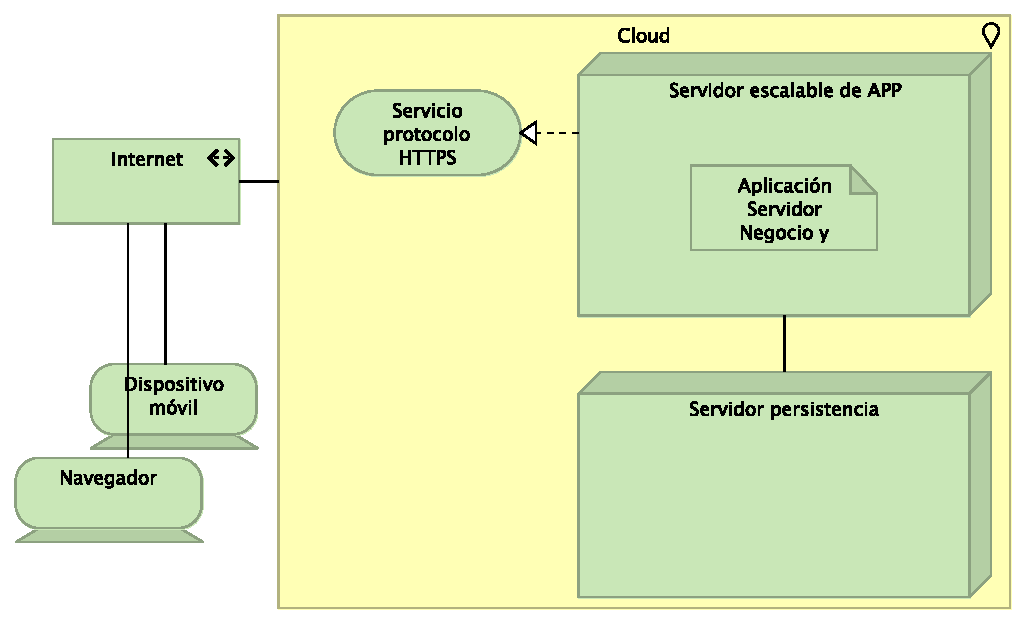
\includegraphics[scale=0.7]{Minfraestructura}
\caption{Punto de vista de infraestructura.}
\label{Minfraestructura}
\end{figure}

\section{Uso de infraestructura}
El punto de vista de uso de infraestructura muestra cómo las aplicaciones son compatibles con la infraestructura de software y hardware: los servicios de infraestructura son entregados por los dispositivos; software y sistemas de redes soportan las aplicaciones. Este punto de vista desempeña un papel importante en el análisis de rendimiento y escalabilidad, puesto que refiere a la infraestructura física para el mundo lógico de aplicaciones. Es muy útil en la determinación de los requisitos de rendimiento y calidad de la infraestructura basada en las exigencias de las diferentes aplicaciones que lo utilizan.

\begin{figure}[H]
\centering
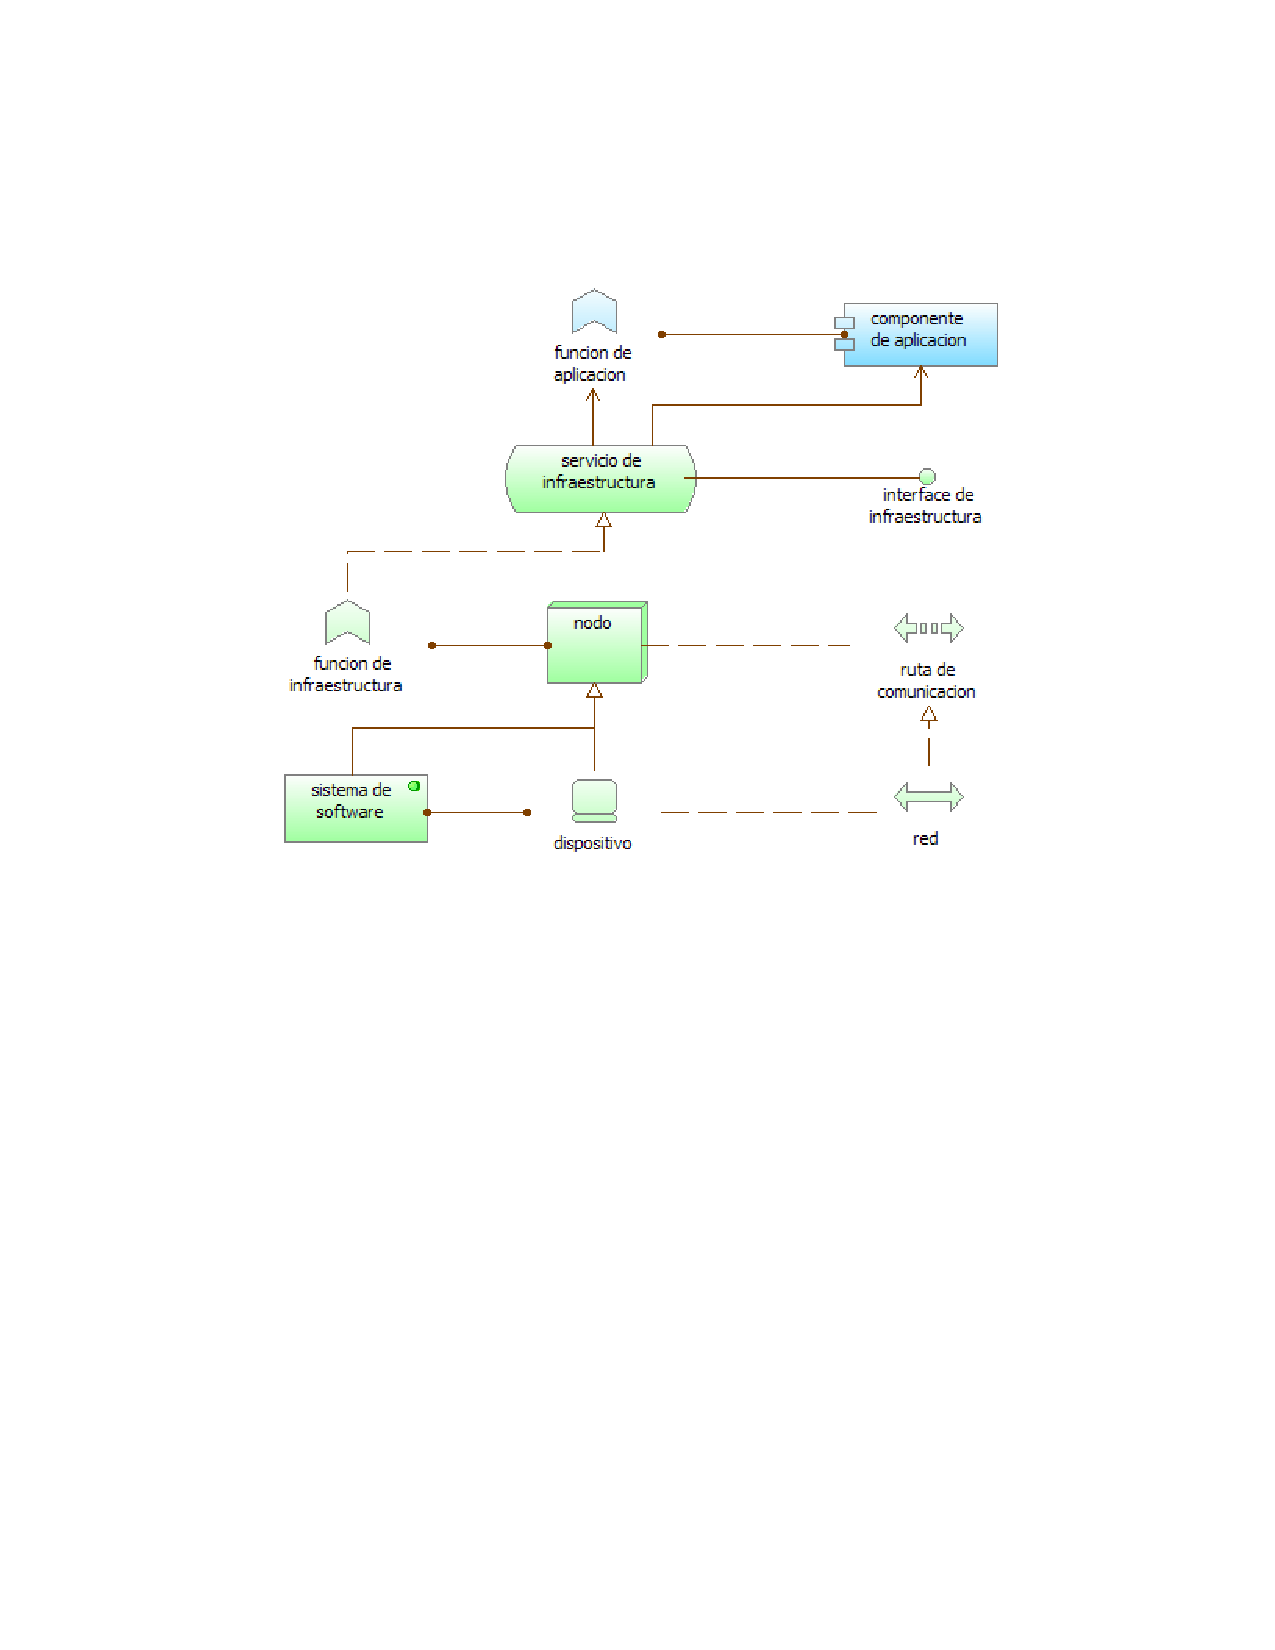
\includegraphics[scale=0.7]{uso_de_infraestructura}
\caption{Metamodelo del punto de vista de uso de infraestructura.}
\end{figure}


\marginpar{
    \begin{figure}[H]
        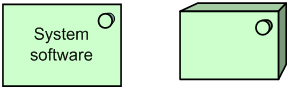
\includegraphics[scale=0.8]{Isystem_software}
    \end{figure} 
    \footnotesize 
    \textbf{Software}. Un entorno de software para tipos específicos de componentes y objetos que son desplegados en forma de artefactos.
\newline
}Los componentes principales de la aplicación estarán distribuidos entre los servicios cloud y el software desplegado en cada dispositivo móvil. Otros elementos no descritos por el punto de vista pueden ser el marketplace: espacio externo para el host de la aplicación antes de ser descargada y el cliente para gestión de información de la marca.

\begin{figure}[H]
\centering
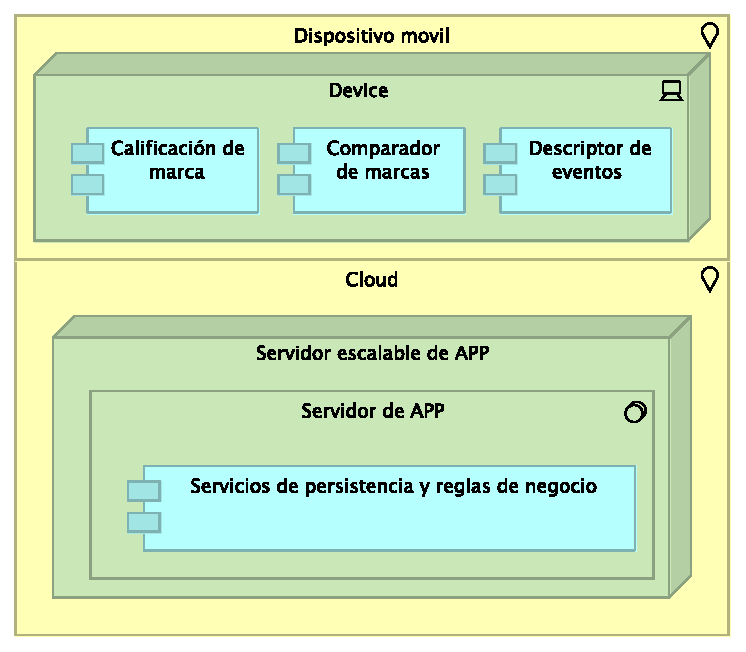
\includegraphics[scale=0.7]{Musoinfraestructura}
\caption{Punto de vista de uso de infraestructura.}
\end{figure}


\marginpar{
    \begin{figure}[H]
        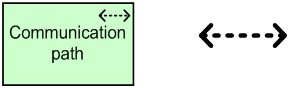
\includegraphics[scale=0.6]{Icommunication_path}
    \end{figure} 
    \footnotesize 
    \textbf{Ruta de comunicación}. Un enlace entre dos o más nodos, a través del cual estos pueden intercambiar datos.
\newline
}

\marginpar{
    \begin{figure}[H]
        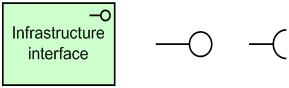
\includegraphics[scale=0.6]{Iinfraestructure_interface}
    \end{figure} 
    \footnotesize 
    \textbf{Interfaz de infraestructura}. Un punto de acceso donde los servicios de infraestructura ofrecidos por un nodo puede ser accedidos por otros nodos y componentes de la aplicación.
}

\section{Despliegue e implementación}
El punto de vista de despliegue e implementación muestra cómo se realizan una o más aplicaciones en la infraestructura. Esto comprende el mapeo de aplicaciones (lógicas) y componentes Onto artefactos (físicas), tales como Enterprise Java Beans, y el mapeo de la información utilizada por estas aplicaciones y componentes sobre la infraestructura de almacenamiento subyacente; por ejemplo, bases de datos o tablas de otros archivos. El punto de vista de implementación juega un papel importante en el análisis de rendimiento y escalabilidad, puesto que refiere la infraestructura física para el mundo lógico de aplicaciones. En seguridad y análisis de riesgos, el punto de vista de implementación se utiliza para identificar, por ejemplo, las dependencias y los riesgos críticos. 

\begin{figure}[H]
\centering
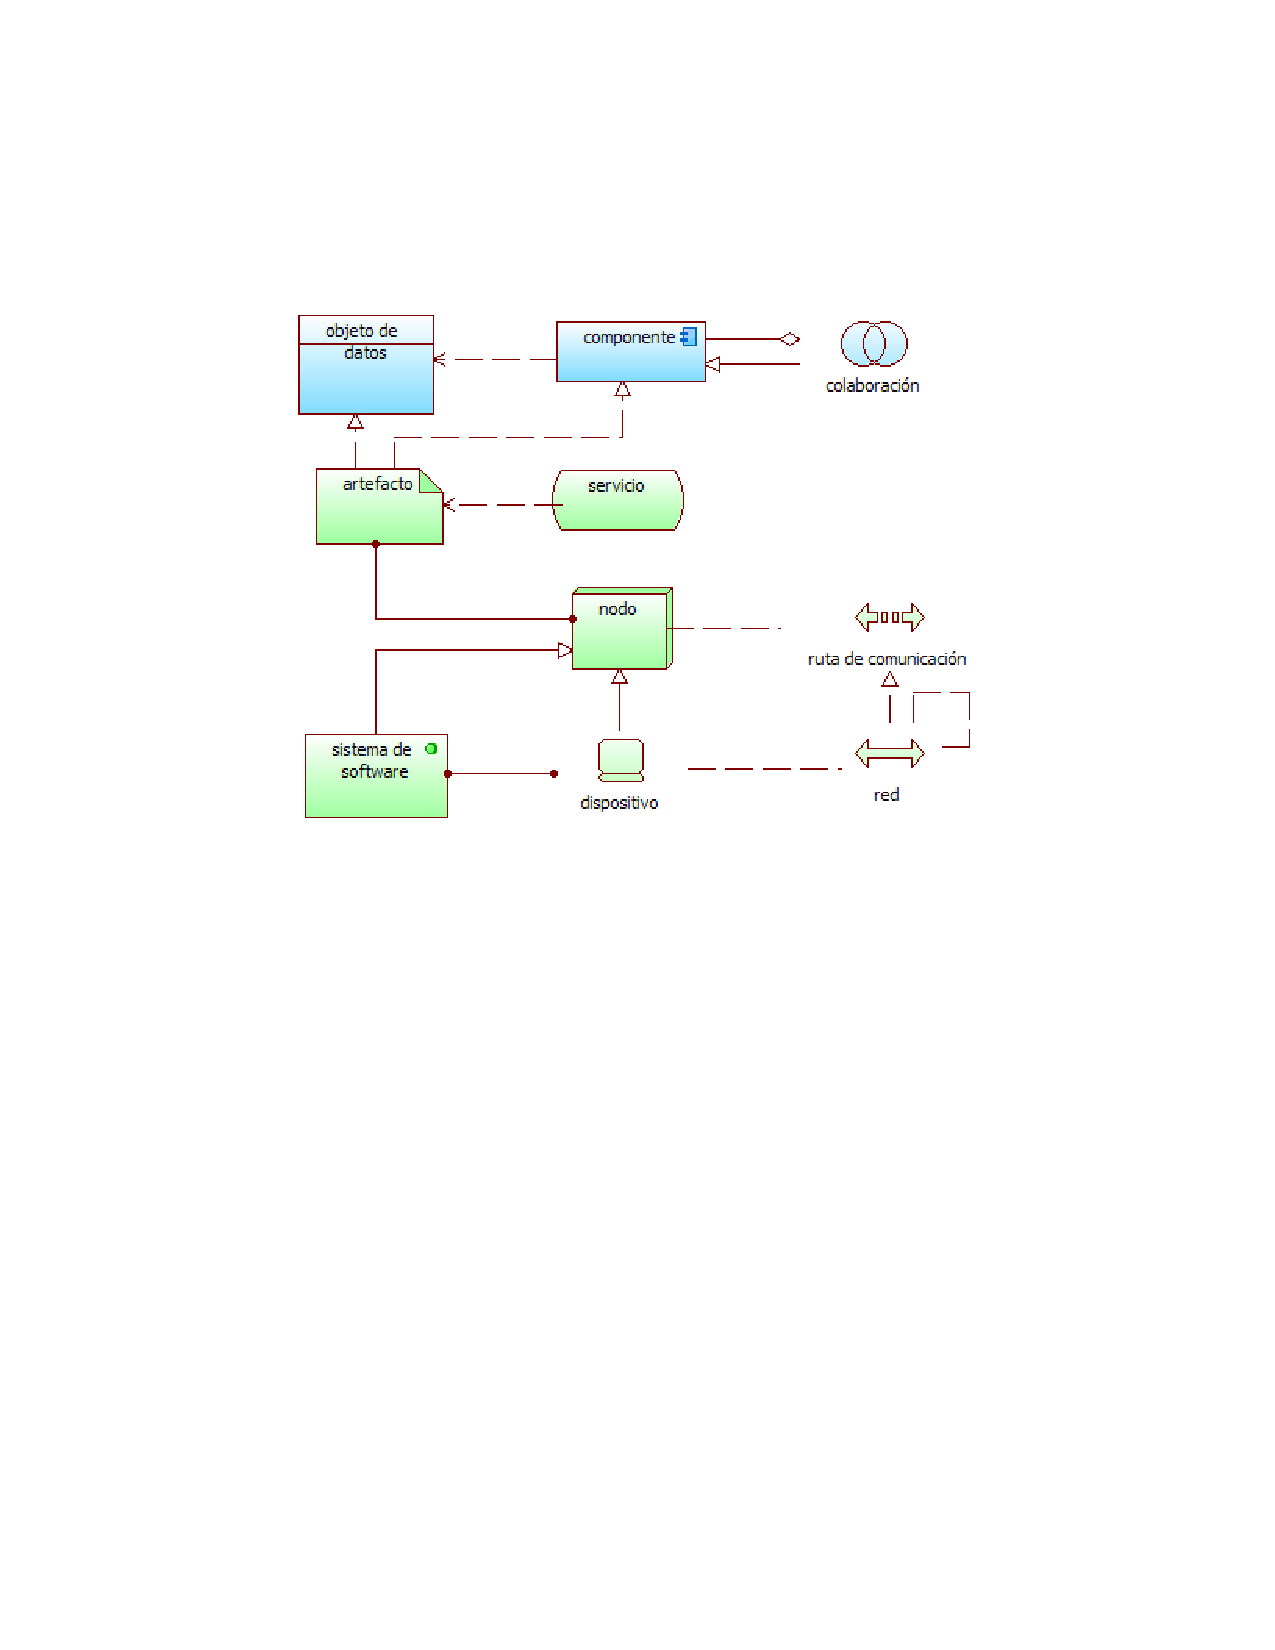
\includegraphics{organizacion_e_implementacion}
\caption{Metamodelo del punto de vista de despliegue e implementación.}
\end{figure}


Es importante destacar que cuando los componentes sean desplegados se comunicarán mediante el protocolo HTTPs sobre el puerto estándar 443.

\begin{figure}[H]
\centering
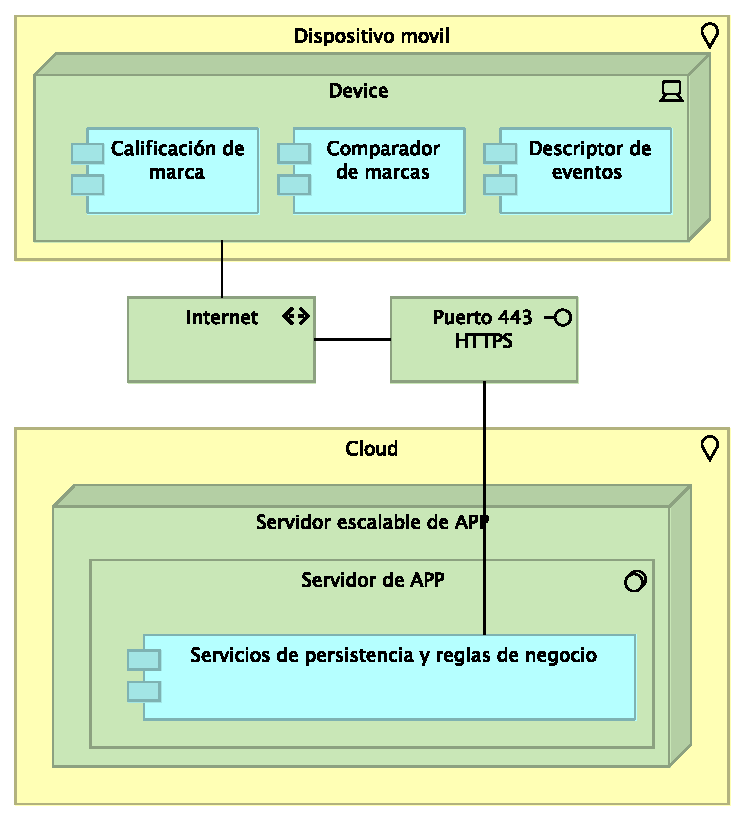
\includegraphics{Mdespliegueimplementacion}
\caption{Punto de vista de despliegue e implementación.}
\end{figure}

\section{Estructura de información}

El punto de vista de estructura de información es comparable a los modelos tradicionales de información creados en el desarrollo de casi cualquier sistema de información. Se muestra la estructura de la información utilizada en la empresa o en un proceso de negocio específico o aplicación, en términos de tipos de datos o las estructuras de clase (orientado a objetos). \marginpar{
    \begin{figure}[H]
        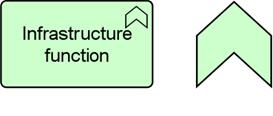
\includegraphics[scale=0.8]{Iinfraestructure_function}
    \end{figure} 
    \footnotesize 
    \textbf{Función de infraestructura}. Un elemento de comportamiento que agrupa un comportamiento de infraestructura que puede ser ejecutado por un nodo.
}
\marginpar{
    \begin{figure}[H]
        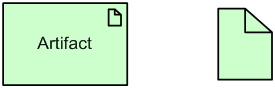
\includegraphics[scale=0.8]{Iartifact}
    \end{figure} 
    \footnotesize 
    \textbf{Artefacto}. Una pieza física de datos que es usada o producida en un proceso de desarrollo de software, o por la implementación y operación de un sistema.
}
Además, puede mostrar cómo la información a nivel empresarial está representado a nivel de aplicación en la forma de las estructuras de datos utilizadas allí, y cómo éstas son entonces mapeadas sobre la infraestructura subyacente; por ejemplo, por medio de un esquema de base de datos.

\begin{figure}[H]
\centering
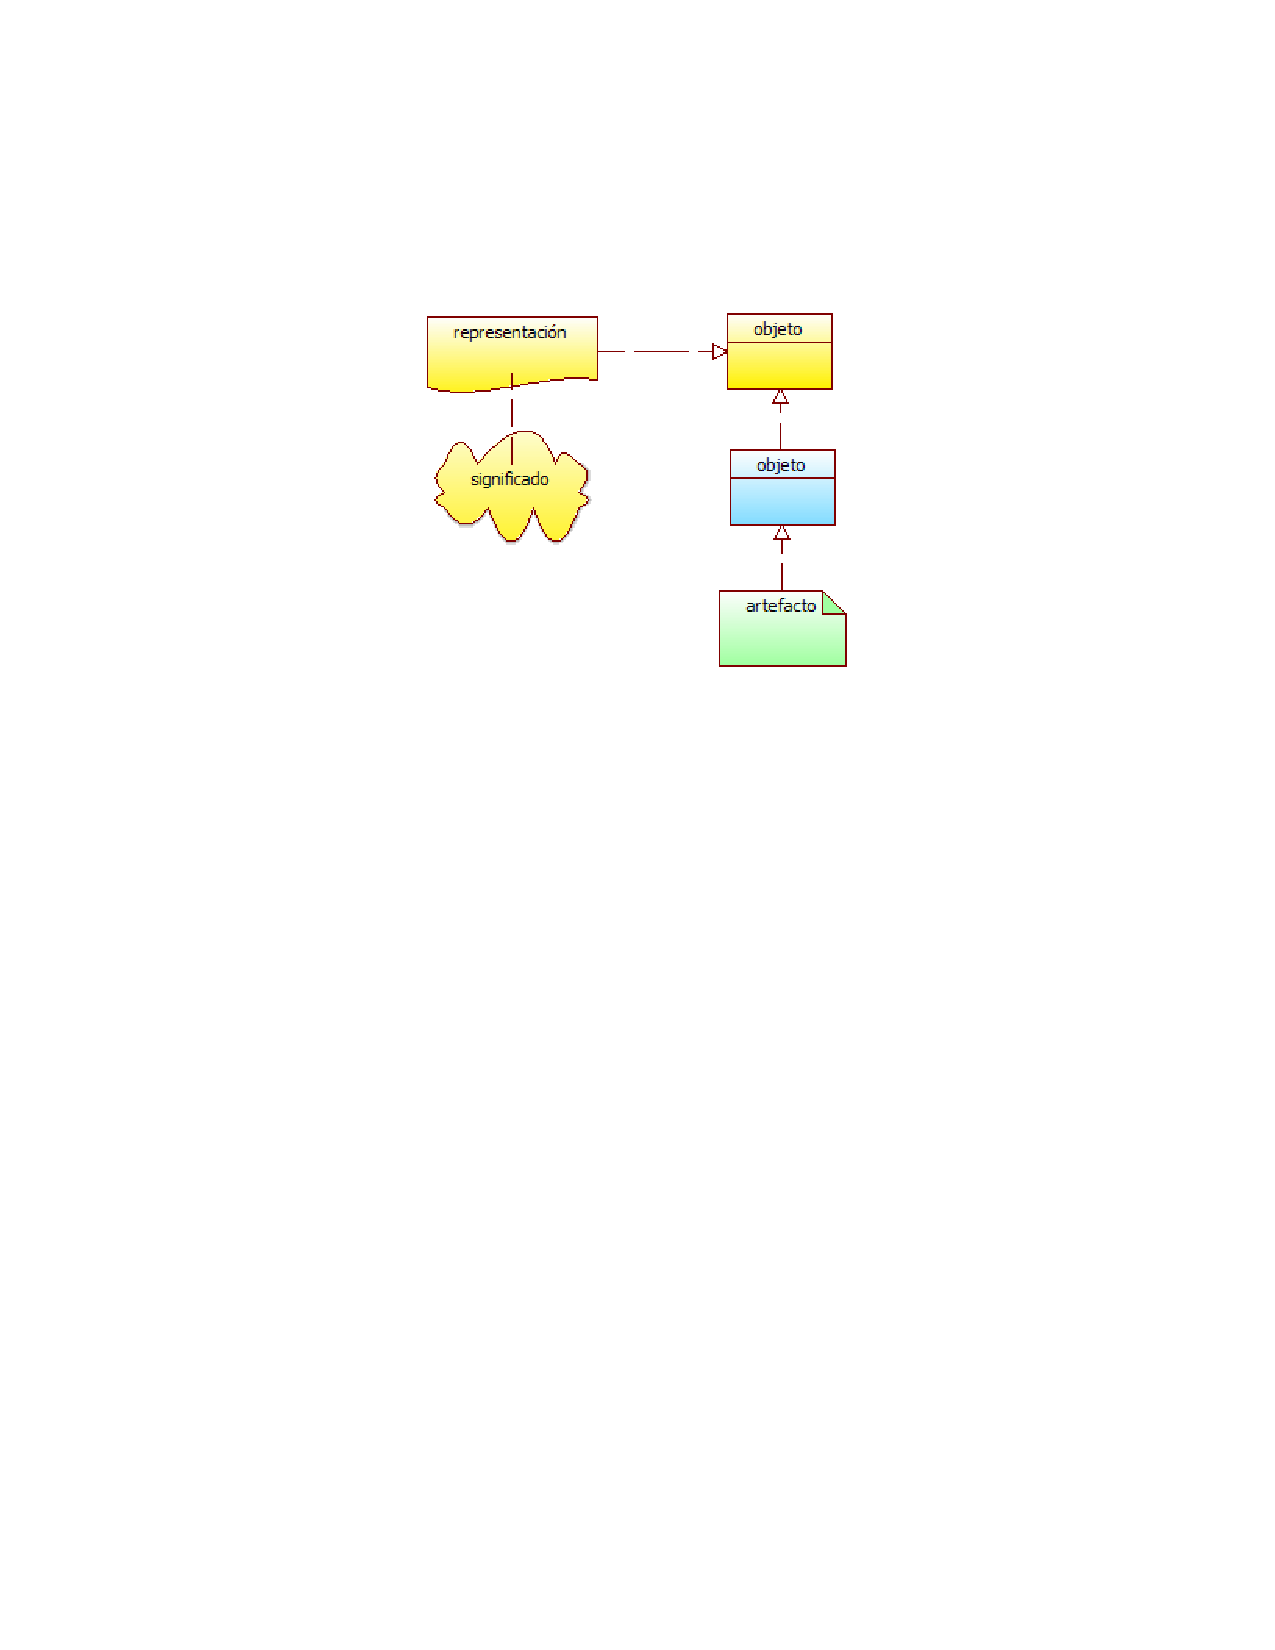
\includegraphics{estructura_de_informacion}
\caption{Metamodelo del punto de vista de estructura de información.}
\end{figure}
Los elementos principales que deben ser modelados son las marcas y sus valoraciones. Adicionalmente las valoraciones deben ser representadas como las calificaciones cuantitativas y las valoraciones en texto o comentarios.

\begin{figure}[H]
\centering
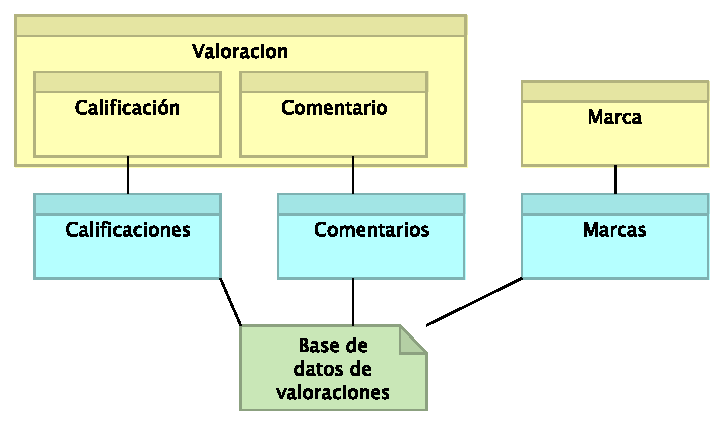
\includegraphics{Mestructurainformacion}
\caption{Punto de vista de estructura de información.}
\end{figure}

\section{Realización del servicio}

\marginpar{
    \begin{figure}[H]
        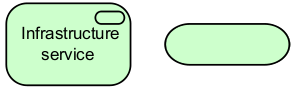
\includegraphics[scale=0.8]{Iinfraestructure_service}
    \end{figure} 
    \footnotesize 
    \textbf{Servicio de infraestructura}. Una unidad visible externa de funcionalidad proporcionada por uno o más nodos, expuesta a través de interfaces bien definidas, y significativa para el entorno.
\newline
}


El punto de vista de realización de servicio se utiliza para mostrar cómo uno o más servicios de negocio se realizan mediante los procesos subyacentes (y algunas veces por componentes de la aplicación). De esta manera, se forma el puente entre el punto de vista de los productos comerciales y de procesos de negocio. Proporciona una "vista desde el exterior" en uno o más procesos de negocio.

\begin{figure}[H]
\centering
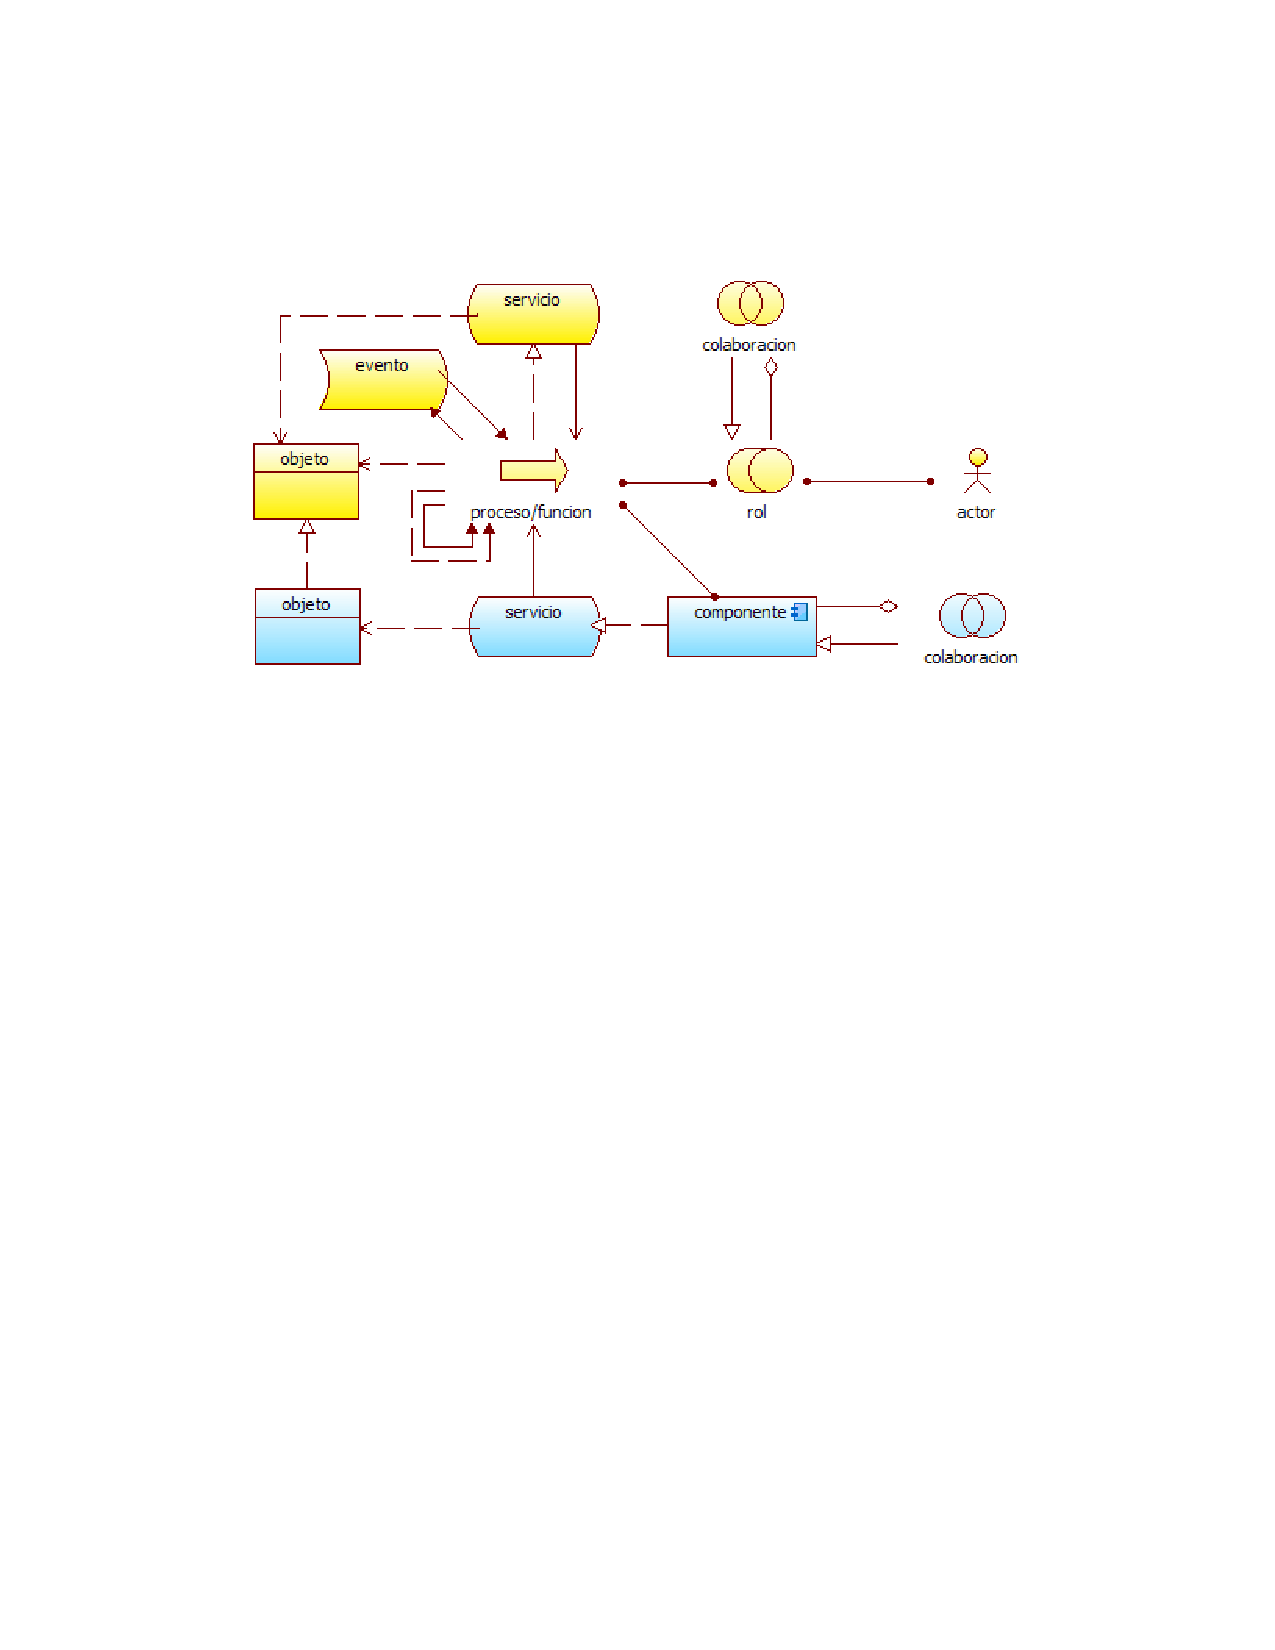
\includegraphics[scale=0.7]{realizacion_del_servicio}
\caption{Metamodelo del punto de vista de realización del servicio.}
\end{figure}

La realización de servicio describe los datos principales que serán gestionados desde la infraestructura montada. En este caso los componentes de software modificarán los datos principales que están descritos en la siguiente figura.

\begin{figure}[H]
\centering
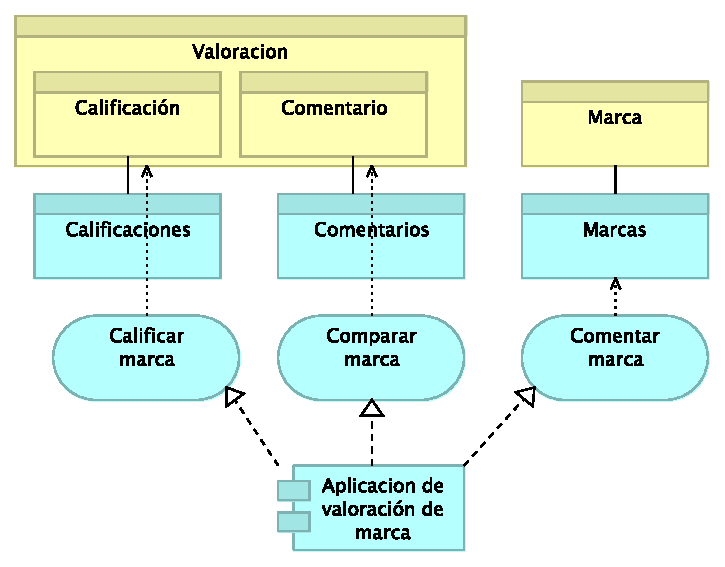
\includegraphics[scale=0.7]{Mrealizacionservicio}
\caption{Punto de vista de realización del servicio.}
\end{figure}

\section{Capas}
El punto de vista en capas dibuja capas y aspectos de una arquitectura empresarial en un diagrama. Hay dos categorías de capas, capas dedicadas y capas de servicio. Las capas son el resultado de la utilización de la relación \textit{agrupación} para una partición natural de todo el conjunto de objetos y las relaciones que pertenecen a un modelo. La infraestructura, la aplicación, el proceso y los actores/roles pertenecen a la primera categoría. El principio estructural detrás de un punto de vista totalmente en capas es que cada capa dedicada expone, por medio de la relación "realización", una capa de servicios, que son más adelante "utilizado por" la siguiente capa dedicada. Por lo tanto, podemos separar fácilmente la estructura interna y la organización de una capa dedicada por parte de su comportamiento observable externamente expresado como la capa de servicio que da cuenta de la capa dedicada. El orden, número, o la naturaleza de estas capas no son fijos, pero en general una (más o menos) de estratificación completa y natural de un modelo ArchiMate deben contener la sucesión de capas descritas. El objetivo principal del punto de vista en capas es proporcionar información general en un diagrama. Además, este punto de vista se puede utilizar como apoyo para el impacto de análisis del cambio y análisis de rendimiento o para la ampliación de la cartera de servicios.

Una descripción transversal para el proyecto es mostrada en la siguiente figura \ref{mcapas}.


\begin{figure}[h]
\centering
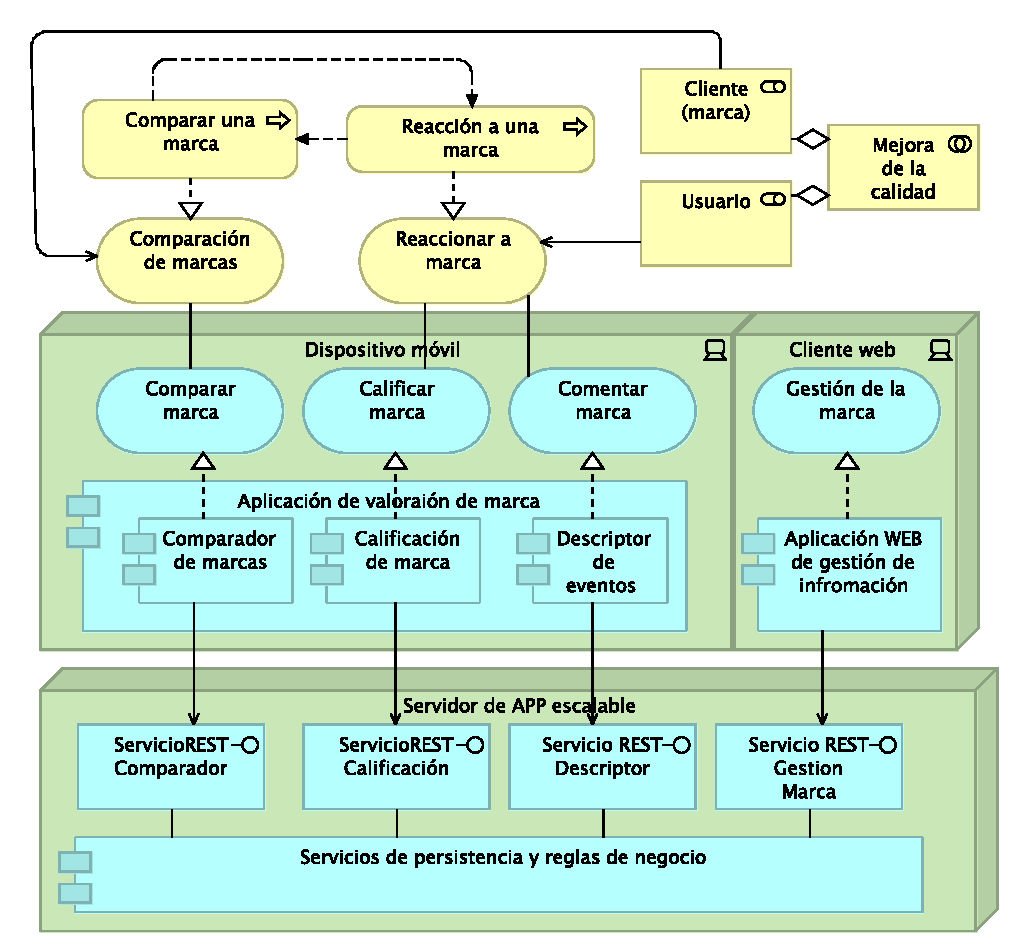
\includegraphics[scale=0.7]{Mcapas}
\caption{Punto de vista de capas.}
\label{mcapas}
\end{figure}
